\section{convergenza integrale}
\label{sec:convergenza_integrale}

Motivati da come viene definita la norma di un vettore
in $\RR^n$ risulta naturale
dare la seguente definizione di
\emph{norma euclidea} per una funzione $f\colon (a,b)\to \RR$:
\[
  \Abs{f}_2 = \sqrt{\int_a^b \abs{f(x)}^2\, dx}.
\]
Questa definizione ha senso, come integrale improprio, se la funzione $f$
è localmente Riemann-integrabile sull'intervallo $(a,b)$
(definizione~\ref{def:localmente_riemann}).
In tal
caso l'integrale esiste, ma potrebbe assumere il valore $+\infty$. Definiamo
allora
\[
\H(a,b) =
\ENCLOSE{\text{$f$ localmente Riemann-integrabile su $(a,b)$}\colon \Abs{ f}_2< +\infty}.
\]

Cercheremo ora di dimostrare che la norma che abbiamo introdotto
è effettivamente un norma (nel senso della definizione~\ref{def:norma})
che rende $\H(a,b)$ uno spazio vettoriale euclideo di dimensione infinita.

Innanzitutto è chiaro che qualunque sia $f$ si ha
$\Abs{ f}_2\ge 0$.
Inoltre è banale osservare che la norma è omogenea: se $t\in \RR$ si ha:
\[
  \Abs{t\cdot f}_2= \abs{t}\cdot \Abs{f}_2.
\]
Dunque se $f\in \H(a,b)$ anche $t f\in \H(a,b)$ per ogni $t \in \RR$.
Se $f,g\in \H(a,b)$ per la proprietà del parallelogramma~\eqref{eq:parallelogramma}
valida in $\RR$ si ha
\[
  (f(x) + g(x))^2 \le 2f^2(x) + 2 g^2(x)
\]
e dunque se $f,g \in \H(a,b)$ anche $f+g\in \H(a,b)$.
Dunque $\H(a,b)$ è uno spazio vettoriale.

Si noti che se $f$ e $g$ sono localmente Riemann-integrabili 
allora anche $f+g$ lo è 
e grazie al teorema~\ref{th:composta_integrabile} anche 
$f^2$, $g^2$ e $(f+g)^2$ lo sono.
Ma allora, anche $f\cdot g = \frac{(f+g)^2-f^2-g^2}{2}$ 
è Riemann-integrabile.
Per $f,g\in \H(a,b)$ possiamo allora definire il prodotto scalare:
\begin{equation}\label{eq:854392}
  \langle f, g\rangle = \int_a^b f(x) \cdot g(x)\, dx.
\end{equation}
La disuguaglianza di
Young~\eqref{eq:Young} valida in $\RR$ ci dice che
\[
  \abs{f(x) \cdot g(x)} \le \frac{f^2(x)+g^2(x)}{2}
\]
e dunque garantisce che l'integrale~\eqref{eq:854392}
sia assolutamente convergente. Dunque se $f,g\in \H(a,b)$
il prodotto scalare $\langle f,g\rangle$ è ben definito ed
è un numero finito. A questo punto è facile verificare
che $\langle f,g\rangle$ è una forma bilineare simmetrica
non negativa. Dunque soddisfa tutte le proprietà formali
date nella definizione~\ref{def:prodotto_scalare} di prodotto scalare
salvo il fatto che non è garantito che $\langle f,f\rangle = 0$
implichi $f=0$. In effetti questa proprietà è falsa perché
se la funzione $f^2(x)$ ha integrale nullo non è detto che sia
identicamente nulla: l'integrale, infatti, non cambia
se la funzione viene modificata in un singolo punto.

Per ovviare a questo problema bisogna che identifichiamo due
funzioni $f,g\in \H(a,b)$ se $\Abs{f-g}_2=0$:
\[
  f \sim g  \iff \Abs{f-g}_2=0.
\]
Chiamiamo $H(a,b)$ il quoziente:
\[
  H(a,b) = \H(a,b)/\sim
\]
cioè lo spazio vettoriale delle funzioni in $\H(a,b)$ dove due funzioni
vengono identificate se la norma della differenza è nulla.

Lo spazio quoziente $H(a,b)$ risulta finalmente essere uno spazio
euclideo.
Mantiene infatti la struttura vettoriale (in quanto l'insieme
delle $f\in \H(a,b)$ con $\Abs{f}_2=0$
è uno spazio vettoriale)
e il prodotto scalare $\langle f,g\rangle$ (e di conseguenza la norma $\Abs{f}_2$)
è ben definito su $H(a,b)$ e oltre alle proprietà che già abbiamo dimostrato
possiamo ora affermare che $\langle f,f\rangle = \Abs{f}_2=0$ se e solo se $f=0$.

\begin{remark}
La notazione $H(a,b)$ che scegliamo di utilizzare per definire questo spazio
non è standard. La lettera $H$ rimanda ad Hilbert in quanto lo studio di questo
spazio in particolare ha spinto verso l'astrazione del concetto di spazio di Hilbert.
Quello che vedremo nel seguito è che questo spazio
non risulta essere completo e dunque in realtà non è uno spazio di Hilbert.
In effetti l'utilizzo degli integrali impropri è un tentativo, di
estendere l'integrale di Riemann in modo da rendere completo questo spazio.
Solo con la definizione di integrale di Lebesgue (1875--1941)
si è riusciti ad estendere l'integrale di Riemann
ad una classe più amplia di funzioni fino a completare lo spazio.
L'analogo dello spazio $H(a,b)$ definito tramite integrale di Lebesgue
viene
usualmente chiamato $L^2$. L'esponente $2$ è dovuto al fatto che
sarebbe possibile definire gli spazi $L^p$
in maniera analoga a quanto fatto nell'esempio~\ref{ex:norma_p}.
Si avrebbe ancora che solo per $p=2$ questi spazi normati sono euclidei,
cioè solo per $p=2$ la norma è indotta da un prodotto scalare.
Tutti gli spazi $L^p$ sono completi e dunque sono spazi di Banach.
Ma $L^2$ è anche uno spazio di Hilbert, in quanto è dotato di prodotto scalare.
Anzi potremmo dire che $L^2$ è lo spazio di Hilbert per antonomasia
e viene denotato anche con il nome $H^0$
(in questo caso l'esponente denota la derivabilità delle funzioni, come
in $C^0$).
\end{remark}

Gli elementi di $H(a,b)$ non sono funzioni, ma classi di equivalenza di funzioni.
Nel seguito, però, tratteremo $f\in H(a,b)$ come se fosse $f\in \H(a,b)$
facendo attenzione che le nostre affermazioni rimangano valide se al posto
di una funzione $f$ si prende una funzione a lei equivalente.
In particolare avrà senso considerare gli integrali di queste funzioni, perché il
valore dell'integrale non dipende dal rappresentante scelto, ma non avrà senso
considerare il valore che le funzioni assumono in un singolo punto, perché
questo dipende dal rappresentante.

\subsection{serie di Fourier}
\index{Fourier!serie di}%
\index{serie!di Fourier}%

Lo spazio $H(a,b)$ è uno spazio vettoriale reale su cui siamo riusciti a definire
un prodotto scalare e quindi una norma. Vorremmo trovare su $H(a,b)$ una base
ortonormale rispetto alla quale sia possibile scrivere le coordinate dei vettori
(cioè delle funzioni) di $H(a,b)$. Visto che $H(a,b)$ non ha dimensione finita
non potremo sperare di trovare una base con un numero finito di elementi.
Introduciamo quindi la seguente.

\begin{definition}[base hilbertiana]
\index{Hilbert!base di}
Sia $V$ uno spazio euclideo. Siano $e_k\in V$ con $k\in \NN$. Diremo che
$e_k$ è un \emph{sistema ortonormale}%
\mymargin{sistema ortonormale}\index{sistema ortonormale} se $\langle e_k, e_j\rangle = 0$ quando
$k\neq j$ e $\langle e_k, e_k\rangle = 1$ per ogni $k\in \NN$.
Diremo che $e_k$ è una \emph{base hilbertiana}%
\mymargin{base hilbertiana}\index{base!hilbertiana} se è un sistema ortonormale
e inoltre per ogni $v\in V$
esistono $c_k\in \RR$ con $k\in\NN$ per cui si abbia
\begin{equation}\label{eq:49346}
  v = \sum_{k=0}^{+\infty} c_k e_k.
\end{equation}
\end{definition}

\begin{theorem}[disuguaglianza di Bessel]
\label{th:bessel}%
Sia $e_0, e_1, e_2, \dots$ un sistema ortonormale in uno spazio euclideo $V$.
Per ogni $v\in V$ e per ogni $k\in \NN$ si ponga $c_k = \langle v,e_k\rangle$.
Allora vale la
\emph{disuguaglianza di Bessel}%
\mymargin{disuguaglianza di Bessel}\index{disuguaglianza!di Bessel}:
\index{Bessel!disuguaglianza di}
\begin{equation}\label{eq:disuguaglianza_Bessel}
\sum_{k=0}^{+\infty} c_k^2 \le \abs{v}^2.
\end{equation}

Vale inoltre l'uguaglianza
\begin{equation}\label{eq:487562}
\sum_{k=0}^{+\infty} c_k^2 = \abs{v}^2
\end{equation}
se e solo se vale la~\eqref{eq:49346}.

Possiamo quindi affermare che il sistema ortonormale $e_0, e_1, e_2, \dots$
è una base hilbertiana se e solo se per ogni $v\in V$ vale l'uguaglianza~\eqref{eq:487562}.
\end{theorem}
%
\begin{proof}
Dato $v\in V$ poniamo $c_k = \langle v,e_k\rangle$ e
\[
   v_N = \sum_{k=0}^N c_k e_k, \qquad w_N = v - v_N.
\]
Osserviamo che per ogni $n\in \NN$ si ha $\langle v_N,w_N\rangle=0$
($w_N$ è ortogonale a $v_N$)
in quanto se $n\le N$:
\[
  \langle w_N , e_n \rangle
  = \langle v, e_n\rangle - \sum_{k=0}^N c_k \langle e_k, e_n\rangle
  = \langle v,e_n\rangle - c_n = 0
\]
e quindi
\[
 \langle w_N, v_N \rangle = \sum_{k=0}^N c_k \langle w_N, e_k\rangle = 0.
\]
dunque possiamo concludere, grazie al teorema di Pitagora~\eqref{eq:Pitagora}
\begin{align*}
  \abs{v}^2
  &= \abs{v_N + w_N}^2
  = \abs{v_N}^2 + \abs{w_N}^2 \\
  &\ge \abs{v_N}^2 = \abs{\sum_{k=0}^N c_k e_k}^2
  = \sum_{k=0}^N c_k^2.
\end{align*}
Passando al limite per $N\to +\infty$ si ottiene la disuguaglianza
di Bessel.

Abbiamo visto che $\abs{w_N}^2 = \abs{v}^2 - \abs{v_N}^2$
dunque la condizione $\abs{w_N}^2\to 0$ è equivalente
all'uguaglianza di Bessel: $\abs{v_N}^2 \to \abs{v}^2$.
Il sistema è hilbertiano, per definizione, se e solo se $v_N \to v$
ovvero se $w_N\to 0$.
\end{proof}

Il nostro obiettivo è ora quello di produrre una base hilbertiana di $H(0,2\pi)$.
Una base di $H(a,b)$ si potrà ottenere di conseguenza traslando e riscalando opportunamente le funzioni della base di $H(0,2\pi)$.
Il teorema precedente ci dice che se $H(a,b)$ ammette una base 
hilbertiana $e_k$ allora 
ogni funzione $u\in H(a,b)$ può essere semplicemente rappresentata 
da una successione numerica $x_k = (u, e_k)$ in modo che 
\[
    \Abs{u}_2 = \sqrt{\sum_k x_k^2}.
\]
\mynote{%
Se $u$ rappresenta l'intensità del segnale acustico emesso da uno 
strumento musicale che suona una certa nota, 
possiamo immaginare che $u$ sia una funzione periodica di frequenza $\nu$ 
pari alla frequenza della nota emessa. 
Le funzioni $e_k$ della base hilbertiana sono funzioni sinusoidali
ognuna con frequenza $\nu k$.
I coefficienti $x_k$ nella decomposizione $u = \sum x_k u_k$ 
rappresentano le intensità di ognuna di queste frequenze fondamentali 
e determinano il \emph{timbro} dello strumento musicale.
}

Consideriamo le seguenti funzioni trigonometriche%
\mynote{%
Dal punto di vista algebrico sarebbe molto più semplice considerare le
funzioni a valori complessi:
\[
  e_k(x) = \frac{e^{ikx}}{\sqrt{2\pi}}
\]
al variare di $k\in \ZZ$. Preferiamo però rimanere nell'ambito delle funzioni
reali per non dover introdurre la struttura hermitiana
degli spazi vettoriali complessi.}%
:
\begin{equation}\label{eq:54741346}
\begin{aligned}
  e_0 (x) &= \frac{1}{\sqrt{2\pi}} \\
  e_{2k+1}(x) &= \frac{\sin(kx)}{\sqrt{\pi}} \qquad k=0,1,\dots\\
  e_{2k}(x) &= \frac{\cos(kx)}{\sqrt{\pi}} \qquad k=1,2,\dots
\end{aligned}
\end{equation}
Ovviamente
\[
  \Abs{e_0}_2=\sqrt{\int_{0}^{2\pi} \enclose{\frac{1}{\sqrt{2\pi}}}^2\, dx} = 1
\]
ma è anche facile verificare che
\[
  \int_{0}^{2\pi} \cos^2 (kx)\, dx
  = \frac{1}{k}\int_{0}^{2k\pi} \cos^2 y\, dy
  = \int_{0}^{2\pi} \cos^2 y\, dy = \pi
\]
da cui si ottiene $\Abs{e_{2k}}_2 = 1$.
Visto che la funzione $\sin$ è la traslata di $\cos$ si
ottiene analogamente che $\Abs{e_{2k+1}}_2=1$.
Dunque i vettori $e_0,e_1,\dots$ sono tutti di modulo unitario.
Utilizzando la formula di Eulero
si può trovare la \emph{formula di Werner}%
\mymargin{formula di Werner}\index{formula di Werner}:
\index{Werner!formula di}%
\index{formula!di Werner}%
\begin{align*}
 \sin(mx)\cos(nx)
 &= \frac{e^{imx}-e^{-imx}}{2i}\cdot \frac{e^{inx}+e^{-inx}}{2}\\
 &= \frac{e^{i(m+n)x}}{4i} - \frac{e^{-i(m+n)x}}{4i} 
  + \frac{e^{i(m-n)x}}{4i} - \frac{e^{-i(m-n)x}}{4i}\\
 &= \frac{\sin\enclose{(m+n)x}}{2} + \frac{\sin\enclose{(m-n)x}}{2}
\end{align*}
da cui se $m\neq n$:
\begin{align*}
 \int_{0}^{2\pi} \sin(mx)\cos(nx)\, dx &=
 -\frac 1 {2(m+n)} \Enclose{\cos\enclose{(m+n)x}}_{0}^{2\pi} \\
  &\quad - \frac{1}{2(m-n)}\Enclose{\cos\enclose{(m-n)x}}_{0}^{2\pi} = 0
\end{align*}
e se $m=n$ si arriva comunque allo stesso risultato.
Questo significa che $\langle e_{2n},e_{2m+1}\rangle = 0$.
Discorso analogo si può fare per le funzioni $\sin(mx)\sin(nx)$ e $\cos(mx)\cos(nx)$
trovando, anche in quei casi, che tali prodotti hanno integrale nullo
nell'intervallo $[0,2\pi]$.
Per nostra memoria le formule di Werner che si trovano
in questi ultimi casi sono:
\mymargin{formule di Werner}%
\index{formule di Werner}%
\index{Werner!formula di}%
\index{formula!di Werner}%
\begin{align*}
  \cos(mx) \cos(nx) &=  \frac{\cos((m+n)x)}{2} + \frac{\cos((m-n)x)}{2}\\
  \sin(mx) \sin(nx) &=  \frac{\cos((m-n)x)}{2} - \frac{\cos((m+n)x)}{2}.
\end{align*}

Risulta dunque che le funzioni $e_0,e_1,e_2,\dots$ definite da~\eqref{eq:54741346}
formano un sistema ortonormale in $H(0,2\pi)$
in quanto si ha:
\[
  \langle e_n, e_m \rangle =
  \begin{cases} 1 &\text{se $m=n$}\\
  0 & \text{altrimenti}.
  \end{cases}
\]
Di conseguenza le funzioni $e_0,e_1,e_2, \dots$ sono tra loro indipendenti
in $H(0,2\pi)$ in quanto se una loro combinazione lineare è nulla:
\[
  \sum_{k=0}^n \lambda_k e_k = 0
\]
allora, facendone il prodotto scalare con $e_j$ si ottiene:
\[
  0 = \langle \sum_{k=0}^n \lambda_k e_k , e_j\rangle
  = \sum_{k=0}^n \lambda_k \langle e_k, e_j\rangle
  = \lambda_j
\]
e dunque tutti i coefficienti $\lambda_j$ sono nulli.
Possiamo in particolare dedurre che $H(0,2\pi)$ ha dimensione
infinita.

\begin{definition}[polinomi trigonometrici]
Una funzione $f$ si dice essere un \emph{polinomio trigonometrico}%
\mymargin{polinomio trigonometrico}\index{polinomio trigonometrico}
se esiste un polinomio in due variabili $P(X,Y)$ tale che
\[
  f(x) = P(\cos x, \sin x).
\]
\end{definition}

Possiamo verificare che $f$ è un polinomio trigonometrico se e solo se
è possibile scrivere $f$ come combinazione lineare finita delle funzioni $e_k$
appena introdotte,
cioè se esistono $c_0, c_1, \dots, c_n\in \RR$ tali che
\[
  f = \sum_{k=0} c_k e_k.
\]
Basta infatti ricondurre le funzioni trigonometriche all'esponenziale complesso,
tramite la formula di Eulero:
\begin{align*}
   \cos(nx) + i \sin(nx)
   &= e^{inx} = (e^{ix})^n
   = \enclose{\cos x + i \sin x}^n\\
   &= \sum_{k=0}^n {n \choose k} i^k \enclose{\sin x}^k \enclose{\cos x}^{n-k}
\end{align*}
da cui, prendendo parte reale, e parte immaginaria si
riesce ad esprimere $\cos(nx)$ e $\sin(nx)$ come polinomio in $\sin x$ e $\cos x$.
Più precisamente per il coseno
si ottengono solo i termini con $k$ pari:
\begin{align*}
\cos(nx) &= \sum_{k=0}^{\floor{\frac n 2}} {n \choose 2k} (-1)^k \enclose{\sin x}^{2k} \enclose{\cos x}^{n-2k}\\
&= \sum_{k=0}^{\floor{\frac n 2}}{n \choose 2k} \enclose{\cos^2 x -1}^k \enclose{\cos x}^{n-2k}
\end{align*}
ovvero
\[
  \cos(nx) = T_n(\cos x)
\]
dove
\[
  T_n(x) = \sum_{k=0}^{\floor{\frac n 2}}{n \choose 2k} \enclose{x^2 -1}^k x^{n-2k}
\]
si chiama \emph{polinomio di Chebyshev di prima specie}.
\index{polinomio!di Chebyshev}%
\index{Chebyshev!polinomio di}%
Questo significa che ognuna delle funzioni $e_k$ che abbiamo introdotto
in~\eqref{eq:54741346} è un polinomio trigonometrico e quindi ogni
combinazione finita di tali funzioni è ancora un polinomio trigonometrico.

Viceversa per verificare che ogni polinomio trigonometrico può essere rappresentato
come combinazione lineare finita degli elementi $e_k$
possiamo osservare che se $f(x) = P(\cos x,\sin x)$ è un polinomio trigonometrico
allora usando le formule di Eulero si può scrivere $f(x) = Q(e^{ix}, e^{-ix})$
dove $Q$ è un polinomio a coefficienti complessi. Ma osservando che
\[
  \enclose{e^{ix}}^n = e^{inx}
\]
si ottiene che $f(x)$ può essere scritta come combinazione lineare complessa
delle funzioni $e^{ikx}$ e $e^{-ikx}$. Utilizzando nuovamente le fomule di
Eulero si deduce che $f(x)$ può essere scritta come combinazione lineare
complessa delle funzioni $\cos(ikx)$ e $\sin(ikx)$:
\[
  f(x) = \sum_{k=0}^n \enclose{z_k \cos(kx) + w_k \sin(kx)}.
\]
Ma visto che sappiamo che $f(x)$ è una funzione reale, la somma delle parti
immaginarie di questa combinazione lineare è nulla e dunque abbiamo ottenuto
che $f(x)$ è combinazione lineare a coefficienti reali
delle funzioni $e_n$.

\begin{definition}[serie di Fourier]
Se $f\in \H(0,2\pi)$ i coefficienti $c_k = \langle f, e_k\rangle$
si chiamano \emph{coefficienti di Fourier}%
\mymargin{coefficienti di Fourier}\index{coefficienti di Fourier} di $f$
e la serie
\[
  \sum_{k=0}^{+\infty} c_k e_k
\]
si chiama \emph{serie di Fourier}%
\mymargin{serie di Fourier}\index{serie!di Fourier} di $f$.
Il polinomio trigonometrico
\[
  f_N = \sum_{k=0}^{N} c_k e_k
\]
si chiama \emph{sviluppo di Fourier}%
\mymargin{sviluppo di Fourier}\index{sviluppo di Fourier} di ordine $N$ per $f$.
\end{definition}

\begin{example}
Calcoliamo lo sviluppo di Fourier della funzione:
\[
  f(x) = 
  \begin{cases}
    1 & \text{se $x\in [0,\pi]$}\\
    -1 & \text{se $x\in (\pi,2\pi]$}.
  \end{cases}
\]
Per quanto riguarda $c_0 = \langle f, e_0\rangle$ si ha
banalmente: 
\[
c_0 = \int_0^{2\pi} f(x) \cdot \frac{1}{\sqrt{2\pi}}\, dx 
  = \frac{1}{\sqrt{2\pi}}\Enclose{\int_0^\pi 1 \, dx + \int_0^\pi (-1)\, dx}
  = 0.  
\]
Per $c_{2k} = \langle f, e_{2k}\rangle$ si ha 
\begin{align*}
  c_{2k}
  &= \int_0^{2\pi} f(x)\frac{\cos (kx)}{\sqrt{\pi}}\, dx \\
  &= \frac{1}{\sqrt \pi} \Enclose{\int_0^\pi \cos (kx)\, dx 
  - \int_{\pi}^{2\pi} \cos(kx)\, dx}
  = 0 
\end{align*}
per motivi di simmetria.
Per calcolare $c_{2k+1}=\langle f, e_{2k+1}\rangle$ 
si trova 
\begin{align*}
  c_{2k+1}
  &= \int_0^\pi \frac{\sin(kx)}{\sqrt \pi}\, dx 
    - \int_\pi^{2\pi} \frac{\sin(kx)}{\sqrt \pi}\, dx \\
  &= \frac{2}{\sqrt \pi}\int_0^\pi \sin(kx)\, dx
  = \frac{2}{k\sqrt \pi}\int_0^{k\pi}\sin t\, dt\\
  &= 
  \begin{cases}
    0 & \text{se $k$ pari,}\\
    \frac{4}{k\sqrt \pi} & \text{se $k$ dispari.}
  \end{cases}
\end{align*}
Si trova quindi che   
\[
 f_{2n+1}(x)
 = \sum_{k=0}^n \frac{4}{(2k+1)\sqrt \pi}\sin((2k+1)x).
\]
Si veda la figura~\ref{fig:fourier}.
\end{example}

\begin{figure}
  \begin{center}
  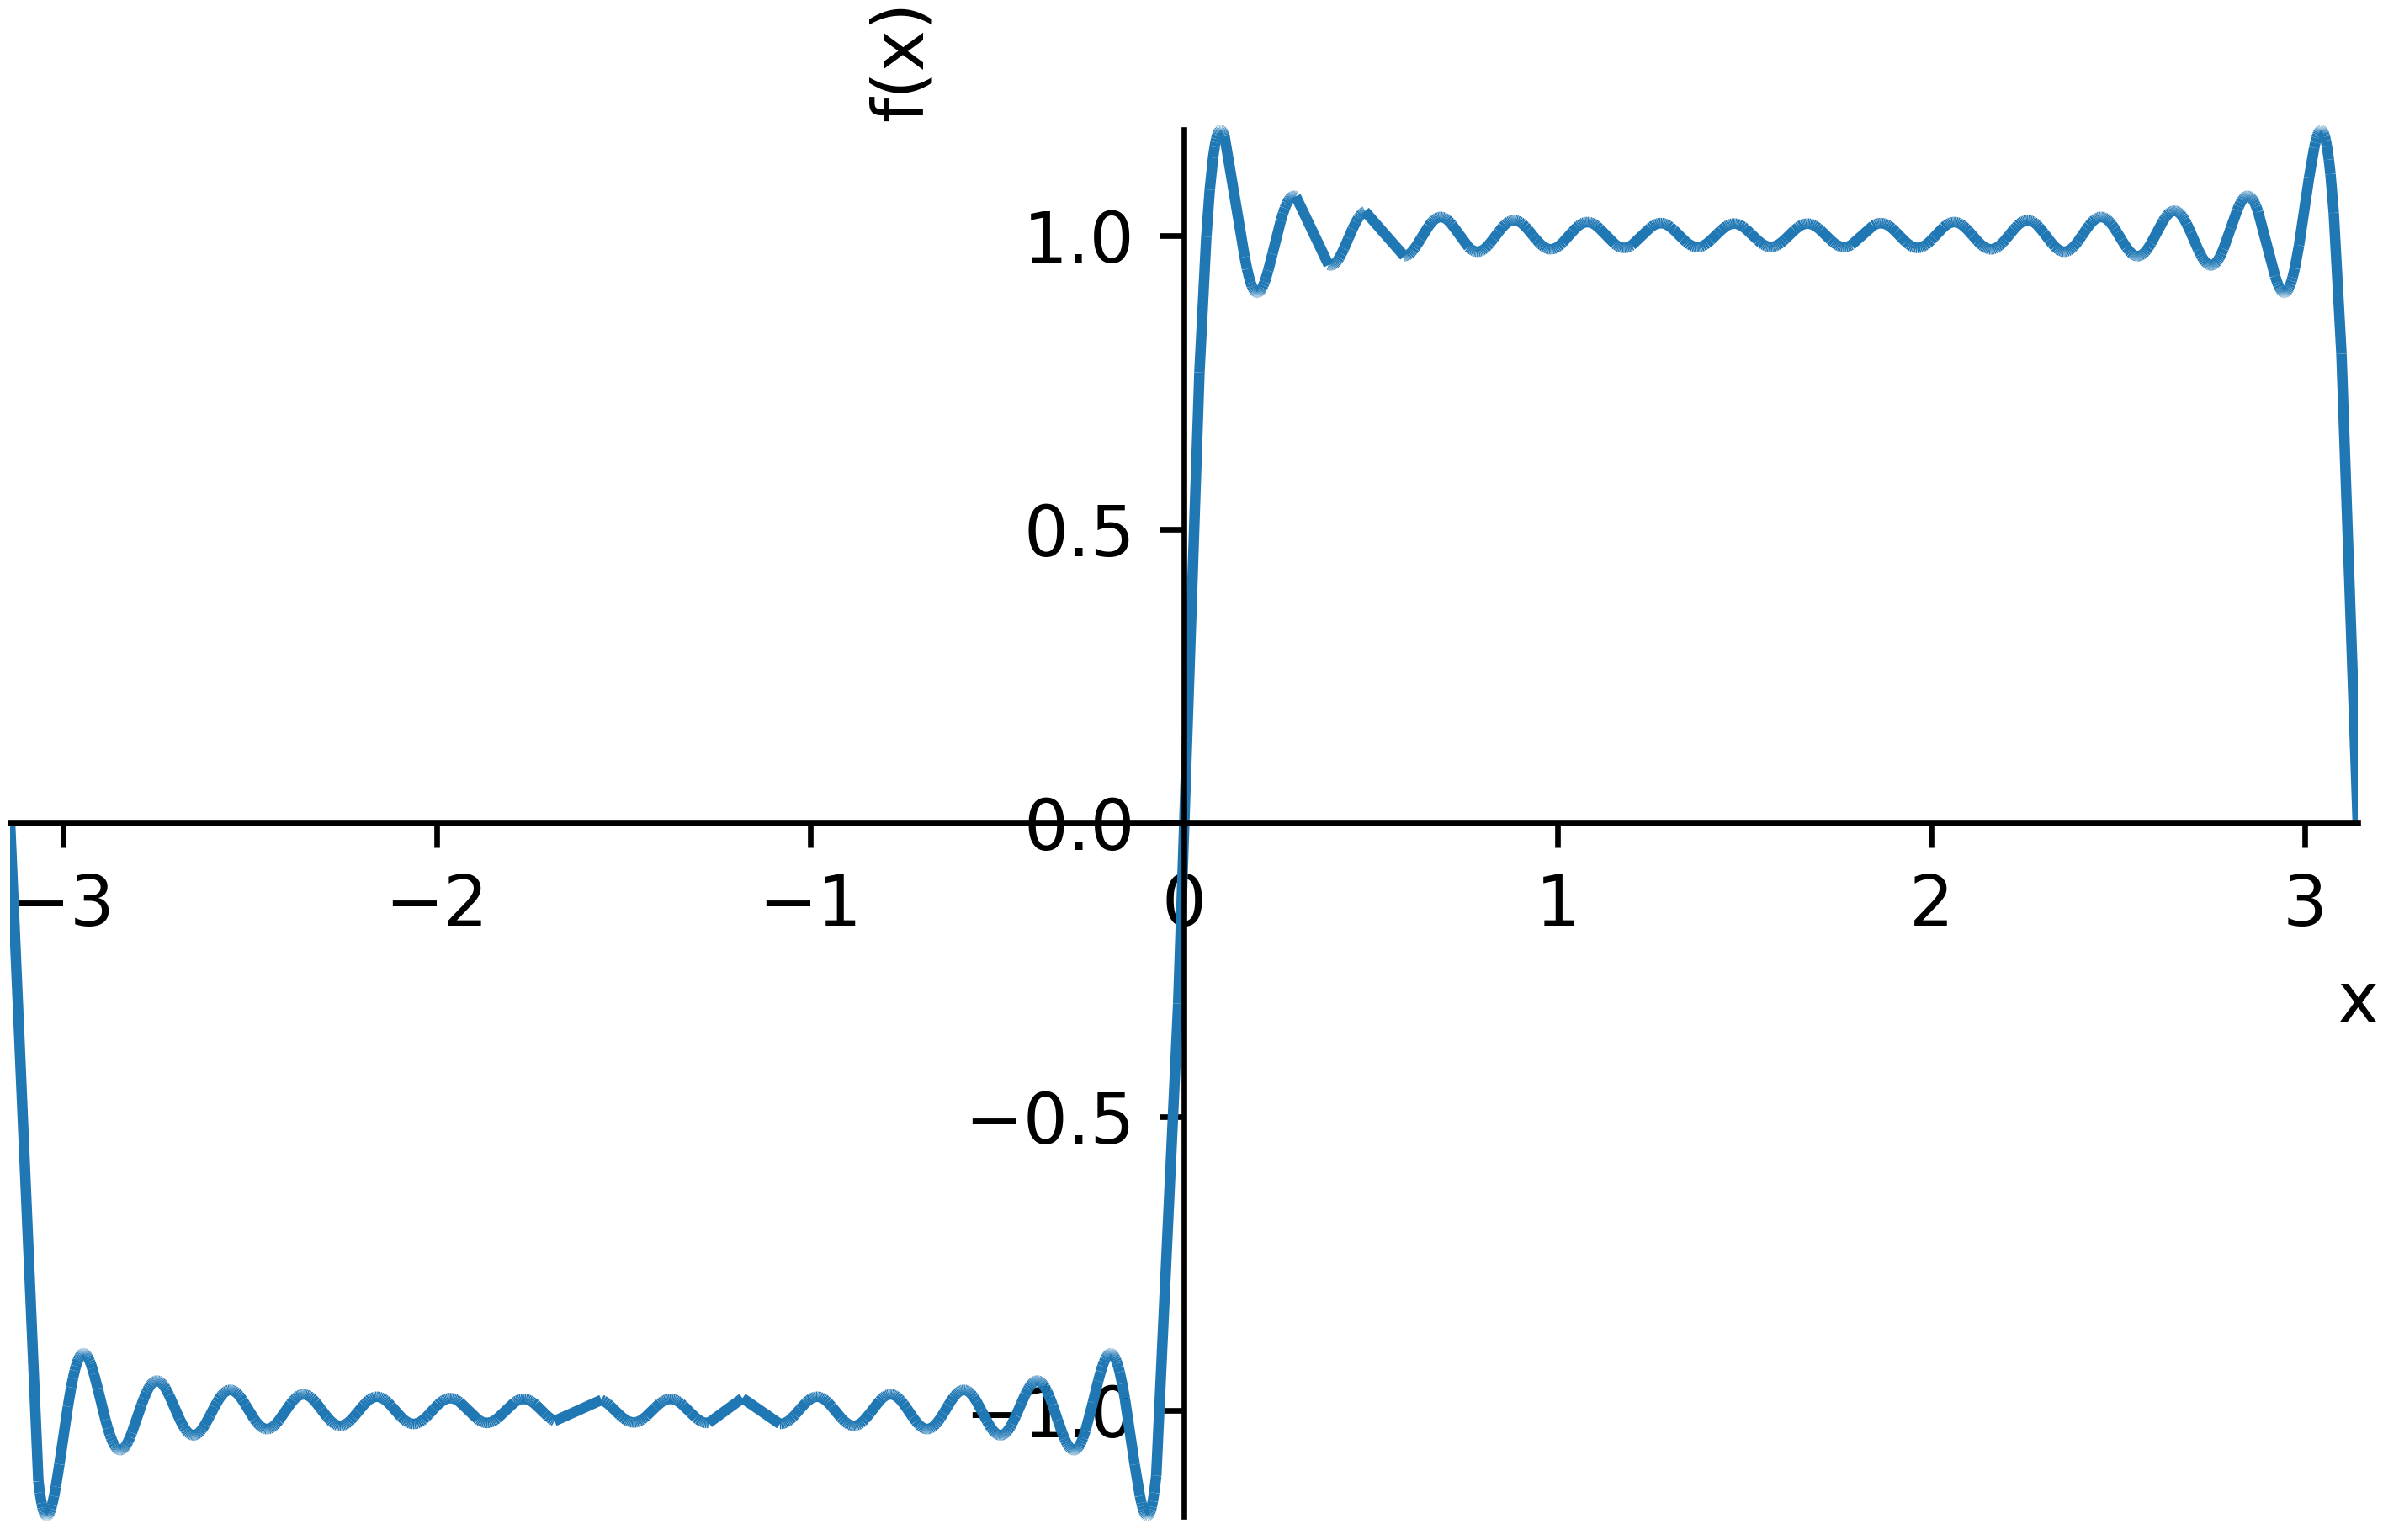
\includegraphics[height=5cm]{fourier.png}
  \end{center}
  \captionsetup{singlelinecheck=off}
  \caption{Lo sviluppo di Fourier della funzione
  che vale $1$ su $[0,\pi]$ e $-1$ su $[\pi,2\pi]$:
  $
  f_{61}(x)=
  \frac{4\sin(x)}{\pi} + \frac{4\sin(3x)}{3\pi} + \frac{4\sin(5x)}{5\pi} + \frac{4\sin(7x)}{7\pi} + \frac{4\sin(9x)}{9\pi} + \frac{4\sin(11x)}{11\pi} + \frac{4\sin(13x)}{13\pi} + \frac{4\sin(15x)}{15\pi} + \frac{4\sin(17x)}{17\pi} + \frac{4\sin(19x)}{19\pi} + \frac{4\sin(21x)}{21\pi} + \frac{4\sin(23x)}{23\pi} + \frac{4\sin(25x)}{25\pi} + \frac{4\sin(27x)}{27\pi} + \frac{4\sin(29x)}{29\pi} + \frac{4\sin(31x)}{31\pi}
  $.
  Il codice per calcolare i coefficienti e generare il grafico
  si trova a pagina~\pageref{code:Fourier}.
  Si può notare come nel punto di salto $x=\pi$ 
  lo sviluppo di Fourier ha una oscillazione maggiore del salto 
  originario (fenomeno di Gibbs).
  \index{Gibbs!fenomeno di}
  \index{fenomeno di Gibbs}
  L'incremento dell'oscillazione è circa del 9\% ed è indipendente 
  dal numero di termini utilizzati nello sviluppo di Fourier.
%  Significa che la serie di Fourier pur convergendo in norma $\Abs{\cdot}_2$
%  non converge uniformemente.
  }
  \label{fig:fourier}
  \end{figure}
    
Risulta naturale chiedersi se quella che abbiamo introdotto è una
\emph{base hilbertiana} perché solo in tal caso gli sviluppi di Fourier
approssimano la funzione.
Per ottenere questo risultato dobbiamo assumere la validità del seguente
teorema, che sarebbe ora troppo lungo dimostrare.

\begin{theorem}[densità dei polinomi trigonometrici]
Per ogni funzione continua $f\in C^0([0,2\pi])$
con $f(0)=f(2\pi)$ esiste una successione $g_k\in \H(0,2\pi)$ 
di polinomi trigonometrici
(cioè combinazioni lineari finite del sistema $\ENCLOSE{e_k}$)
tale che $g_k$ converge uniformemente a $f$.

In particolare l'insieme dei polinomi trigonometrici
è denso, con la norma uniforme,
nel sottospazio vettoriale
\[
  C^0_0([a,b]) 
  = \ENCLOSE{u\in C^0([a,b])\colon u(a)=u(b)=0}
  \subset C^0([a,b]).
\]
\end{theorem}

Osserviamo che la convergenza uniforme è più forte della convergenza
in $H(a,b)$ in quanto si ha, banalmente:
\[
  \Abs{f}_2^2 = \int_a^b f(x)^2\, dx
  \le \int_a^b \Abs{f}_\infty^2\, dx
  = (b-a) \cdot \Abs{f}_\infty^2.
\]
Dunque il teorema precedente garantisce che ogni funzione continua
in $\H(a,b)$ può essere approssimata, rispetto alla norma $\Abs{\cdot}_2$,
tramite polinomi trigonometrici. Il teorema seguente ci permette
di estendere questa proprietà a tutte le funzioni di $\H(a,b)$.

\begin{theorem}[densità delle funzioni continue]
Data una qualunque $f\in H(a, b)$ per ogni $\eps>0$
esiste una funzione continua $g\colon [a,b]\to \RR$
con $g(a)=g(b)=0$ tale che $\Abs{f-g}_2<\eps$.

Detto in altri termini: $C^0_0([a,b])=\ENCLOSE{u\in C^0\colon u(a)=u(b)=0}$ è un 
sottospazio denso in $H(a,b)$
cioè un insieme la cui chiusura (nella topologia di $H(a,b)$) 
è tutto $H(a,b)$.
\end{theorem}
%
\begin{proof}
\emph{Passo 1. Supponiamo che $f$ sia limitata su $(a,b)$.}
In tal caso possiamo pensare che $f$ sia definita su $[a,b]$
e l'integrale sia un integrale di Riemann ``proprio''.
Sia $M=\sup \abs{f}([a,b])$.
Per le condizioni di integrabilità sappiamo che per ogni $\eps>0$ è possibile
trovare una suddivisione $a=x_0 < x_1 < \dots < x_n =b$ su cui l'integrale
di $f$ differisce dagli integrali superiore e inferiore per meno di $\frac{\eps}{2M}$.
Possiamo prendere come funzione $g$ una interpolazione lineare
cioè una funzione tale che si abbia $g(x_k) = f(x_k)$ sui punti della suddivisione
e che risulti lineare su ogni intervallino $[x_k,x_{k+1}]$. La funzione
$g$ così definita è compresa, su ogni intervallino, tra l'$\inf$ e il $\sup$
di $f$ e dunque si avrà:
\[
 \int_a^b \abs{f(x)-g(x)}\, dx < \frac{\eps}{M}.
\]
Visto però che $\Abs{f}_\infty\le M$
si ha anche $\Abs{g}_\infty\le M$ e quindi $\Abs{f-g}_2\le 2M$.
Ma allora
\[
  \Abs{f-g}_2^2 = \int_a^b \abs{f-g}^2
  \le \int_a^b \Abs{f-g}_\infty \cdot \abs{f(x)-g(x)}\, dx
  \le 2M \frac{\eps}{2M} = \eps.
\]

\emph{Passo 2. Caso generale.}
Se la funzione è assolutamente 
integrabile in senso improprio su $(a,b)$ ma non è limitata, per
definizione di integrale improprio per ogni $\eps>0$ possiamo trovare un intervallo
$[\alpha,\beta]\subset (a,b)$
su cui $f^2$ (e quindi $f$) risulta limitata e
l'integrale di $f^2$ su $(a,\alpha]$ e su $[\beta,b)$
è minore di $\eps$. 
Sia $M=\sup \abs{f}([\alpha,\beta])$.
Applicando il passo precedente sull'intervallo $[\alpha,\beta]$ 
otteniamo una funzione continua $g$ definita su $[\alpha,\beta]$ 
tale che $\abs{g(x)}\le M$
e $\int\abs{f-g}^2\le \eps$.
L'idea è ora di prendere un punto $\alpha'\in(a,\alpha)$ 
e un punto $\beta'\in(\beta,b)$ ed estendere la funzione 
$g$ su tutto $[a,b]$ ponendo $g=0$ sugli intervalli 
$[a,\alpha']$ e $[\beta',b]$ e facendo una interpolazione 
lineare sugli intervalli $[\alpha',\alpha]$ e $[\beta,\beta']$.

Usando la disuguaglianza 
$(f-g)^2 \le (f-g)^2+(f+g)^2 = 2f^2+2g^2$
(si potrebbe altrimenti usare Cauchy-Schwarz due volte)
e scegliendo $\alpha'$ molto vicino ad 
$\alpha$ in modo che si abbia $\alpha-\alpha'<\eps/M^2$,
otteniamo
\[
  \int_a^\alpha \abs{f-g}^2 
  = \int_a^{\alpha'} f^2 + \int_{\alpha'}^\alpha \abs{f-g}^2
  \le \eps + 2\eps + 2M^2\cdot(\alpha-\alpha')
  \le 5\eps.
\]
Disuguaglianza analoga si avrà sull'intervallo $[\beta,b]$.
Dunque otteniamo in conclusione 
\[
\int_a^b \abs{f-g}^2
\le 5\eps + \eps + 5\eps  = 11 \eps
\]
e il teorema è dimostrato con $11\eps$ al posto di $\eps$.
\end{proof}

Grazie ai due teoremi precedenti sappiamo che ogni $f\in \H(a,b)$ può essere
approssimata da polinomi trigonometrici $g_N\to f$
cioè da funzioni della forma:
\[
  g_N = \sum_{k=0}^{N} a_{k,N} e_k.
\]
Stiamo qui assumendo che il polinomio trigonometrico $g_N$ abbia ordine non superiore
ad $N$, ma questo si può sempre assumere, scartando
o ripetendo i termini della successione.

Se ora consideriamo gli sviluppi di Fourier:
\begin{equation}\label{eq:48948784}
  f_N = \sum_{k=0}^N c_k e_k, \qquad c_k = \langle f,e_k\rangle
\end{equation}
ci ricordiamo che per ogni $k\le N$ risulta
\[
   \langle f-f_N, e_k \rangle
   = \sum_{k=0}^N \enclose{\langle f,e_k\rangle - c_k} = 0
\]
e quindi
\[
  \langle f-f_N , g_N -f_N\rangle
  = \sum_{k=0}^N \langle f-f_N, (a_{k,N}-c_k) e_k \rangle
  = 0.
\]
Dunque, applicando il teorema di Pitagora~\ref{th:spazio_euclideo},
\[
  \Abs{f-f_N}_2^2 = \Abs{f-g_N}_2^2 - \Abs{f_N-g_N}_2^2
  \le \Abs{f-g_N}_2^2 \to 0.
\]

Grazie al teorema~\ref{th:bessel} abbiamo quindi ottenuto il seguente.
\begin{theorem}[serie di Fourier]
Se $f\in \H(0,2\pi)$ e $c_k$, $f_N$
sono definiti da~\eqref{eq:48948784}
allora $f_k\to f$ in norma $\Abs{\cdot}_2$.
In particolare vale l'uguaglianza di Bessel
\begin{equation}\label{eq:uguaglianza_Bessel}
  \sum_{k=0}^{+\infty} c_k^2 = \Abs{f}_2^2.
\end{equation}
\end{theorem}


Questo significa, dunque, che il sistema ortonormale che abbiamo introdotto
è una base hilbertiana e quindi che ogni funzione $f\in \H(0,2\pi)$
si approssima
rispetto alla norma $\Abs{\cdot }_2$ con gli sviluppi di Fourier.

Ricordiamo che se $\Abs{f_N-f}_2 \to 0$ non è detto che si abbia la convergenza
puntuale $f_N(x)\to f(x)$ per ogni $x\in (0,2\pi)$ in quanto il limite è unico
in $H(a,b)$ ma non in $\H(a,b)$ e dunque è possibile (e in effetti può succedere)
che il limite puntuale degli sviluppi di Fourier differisca, in alcuni punti,
dalla funzione che si sta approssimando.

Purtroppo lo spazio $H(a,b)$ non risulta essere
completo, come si può vedere nel seguente esempio.

\begin{example}[razionali ingrassati]
\label{ex:incompletezza_di_H}%
Dimostriamo che lo spazio $H(0,1)$ non è completo.

Sappiamo che l'insieme $[0,1]\cap \QQ$ è numerabile, quindi esiste una
successione $q_k$ che elenca tutti i numeri razionali nell'intervallo $[0,1]$.
Poniamo inoltre $r_k = \frac{1}{4\cdot 2^k}$ e consideriamo gli intervalli
$I_k = [q_k-r_k,q_k+r_k]$.
Prendiamo la successione di funzioni $f_n\colon [0,1]\to \RR$
definita da
\[
  f_n(x) =
  \begin{cases}
  1 &\text{se } x\in\displaystyle\bigcup_{k=1}^{n} I_k\\
  0 & \text{altrimenti}
  \end{cases}
\]
A differenza di quanto uno potrebbe pensare, queste funzioni $f_n$ non diventano
mai identicamente uguali ad $1$. Anzi, si può osservare che
\[
  \int_0^1 f_n(x)\, dx
  \le \sum_{k=1}^n \int_{q_k-r_k}^{q_k+r_k} 1\, dx
  = \sum_{k=1}^n \frac{1}{2\cdot 2^k}
  \le \frac{1}{2}\sum_{k=1}^{+\infty}\frac{1}{2^k} = \frac 1 2.
\]

Si può mostrare che $f_k$ è una successione di Cauchy in $H(0,1)$ e
che però non converge in $H(0,1)$.
\end{example}

\begin{proof}
Per verificare che $f_n$ è una successione di Cauchy possiamo semplicemente
osservare che se $n\ge m$ risulta che $f_n$ e $f_m$ differiscono solamente
sugli intervalli $I_k$ con $k$ compreso tra $m$ ed $n$. Dunque:
\[
  \int_0^1 \abs{f_n - f_m}
  \le \sum_{k=m+1}^{+\infty} \int_{q_k-r_k}^{q_k+r_k} 1\,dx
  = \sum_{k=m+1}^{+\infty}\frac{1}{2\cdot 2^k} = \frac{1}{2^{m+1}}.
\]
Visto che $f_n$ e $f_m$ assumono solamente i valori $0$ e $1$ anche $\abs{f_n-f_m}$
assume solamente i valori $0$ e $1$ quindi $\abs{f_n-f_m}^2=\abs{f_n-f_m}$.
Abbiamo quindi verificato che per $n\ge m$ si ha:
\[
  \Abs{ f_n - f_m}_2 \le \sqrt{\frac{1}{2^{m+1}}}.
\]
E' dunque chiaro che comunque sia scelto $\eps>0$ possiamo scegliere $N$
tale che $1/2^N \le \eps^2$ da cui si ottiene che se $n,m\ge N$
allora $\Abs{f_n-f_m}_2 \le \eps$. Cioè: $f_n$ è una successione di Cauchy.

Supponiamo ora, per assurdo, che esista $f\in H(0,1)$
tale che $\Abs{f_n-f}_2 \to 0$.
Innanzitutto visto che ogni $f_k\le 1$ possiamo supporre che sia anche $f\le 1$
perché altrimenti potremmo prendere $g(x) = \min\ENCLOSE{f(x),1}$ e avremmo
chiaramente $\Abs{f_n - g}_2 \le \Abs{f_n -f}_2 \to 0$. In pratica stiamo dicendo
che modificando la funzione $f$ senza cambiarne l'integrale possiamo suppore
che $f(x)\le 1$ per ogni $x\in[0,1]$.

Fissato un intervallo $I_n$, per $k\to +\infty$ si ha:
\[
  0\le \int_{q_n-r_n}^{q_n+r_n}\abs{f_k(x)-f(x)}^2\, dx
  \le \int_0^1 \abs{f_k(x)-f(x)}^2\, dx = \Abs{ f_k -f}_2^2 \to 0.
\]
Ma ora se $k\ge n$ risulta che $f_k=1$ su $I_n$ e quindi il valore dell'integrale
precedente non dipende da $k$ e dovrà quindi essere identicamente nullo:
\[
  \int_{q_n-r_n}^{q_n+r_n} (1-f(x)) \, dx = 0
\]
e quindi possiamo affermare che $\sup f(I_n) = 1$ in quanto se fosse
$\sup f(I_n) = \lambda < 1$
l'integrale di $1-f(x)$ sarebbe positivo
sull'intervallo $I_n$.

Vogliamo ora dimostrare che su ogni intervallo $[a,b]\subset[0,1]$, se $b>a$
si ha $\sup f([a,b])=1$. 
Prendiamo $N$ abbastanza grande in modo che $r_N < (b-a)/3$.
Allora l'intervallo $[a+r_N, b-r_N]$ ha ampiezza maggiore di $r_N$ e contiene infiniti
numeri razionali. 
Esistono quindi infiniti indici $n$ per cui $q_n$ sta in tale
intervallo. 
Tra questi infiniti certamente ce n'è uno con indice $n\ge N$
(perché i $q_n$ con $n<N$ sono in numero finito). 
Ma se $q_n \in [a+r_N,b-r_N]$
allora $I_n\subset[a,b]$ e quindi $\sup f([a,b])\ge \sup f(I_n) = 1$.

Questo significa che per ogni suddivisione di Riemann dell'intervallo $[0,1]$
risulta che il $\sup$ di $f$ sugli intervallini della suddivisione è $1$ e quindi
l'integrale superiore di $f$ è anch'esso $1$. 
Dunque, essendo $f$ integrabile,
\[
  \int_a^b f(x) = 1.
\]

Vogliamo ora concludere che questo è in contraddizione con la disuguaglianza
\[
  \int_a^b f_n(x) \le \frac 1 2
\]
che abbiamo osservato all'inizio.
Si ha infatti per la disuguaglianza di Cauchy-Schwarz
\begin{align*}
  \int_0^1 \abs{f(x)-f_n(x)}\, dx
  \le \Abs{f-f_n}_2\cdot \Abs{1}_2  \to 0
\end{align*}
e quindi, per il criterio di convergenza assoluta,
\[
  \int_0^1 (f(x) - f_n(x))\, dx \to 0.
\]
Ma abbiamo visto che
\[
  \int_0^1 (f(x) - f_n(x))\, dx
  = \int_0^1 f(x)\, dx - \int_0^1 f_n(x)\, dx
  \ge 1 - \frac 1 2 = \frac 1 2
\]
ottenendo quindi un assurdo.
\end{proof}

Il fatto di avere trovato una base hilbertiana di $H(0,2\pi)$ (e quindi
di ogni $H(a,b)$) ci permette di
dire che ogni funzione in $H(0,2\pi)$ può essere rappresentata dalle sue
coordinate $c_k$ in modo che valga l'uguaglianza di Bessel:
\[
  \Abs{f}_2 = \sqrt{\sum_{k=0}^{+\infty} c_k^2}.
\]
Abbiamo in effetti definito una corrispondenza:
\[
  \phi \colon H(0,2\pi) \to \ell^2,
  \qquad
  \ell^2=\ENCLOSE{c\in \RR^\NN \colon \sum_{k=0}^{+\infty} c_k^2<+\infty}
\]
definita da
\[
  c_k = \phi(f) = \langle f, e_k\rangle.
\]
Chiaramente tale $\phi$ è lineare. Visto che $e_k$ è una base hilbertiana
è facile verificare che $\phi$ è anche iniettivo. Se su $\ell^2$
definiamo il prodotto scalare e la norma corrispondente:
\[
  \langle x,y\rangle = \sum_{k=0}^{+\infty} x_k y_k, \qquad
  \abs{x}_2 = \sqrt{\sum_{k=0}^{+\infty}} x_k^2
\]
l'uguaglianza di Bessel ci dice che $\phi$ mantiene la norma e quindi
la struttura di spazio euclideo. Si potrebbe dimostrare che $\ell^2$
è completo e questo significa che $\phi$ non è suriettiva in quanto
la successione $f_n$
considerata nell'esempio~\ref{ex:incompletezza_di_H}
è di Cauchy in $H(0,2\pi)$, dunque $\phi(f_n)$ è di Cauchy in $\ell^2$
e dunque converge in $\ell^2$. Il limite $c$ della successione $\phi(f_n)$
rappresenta una successione di coefficienti di Fourier che non possono
essere ottenuti da nessuna funzione $f\in H(0,2\pi)$.

Possiamo utilizzare le serie di Fourier per risolvere 
il seguente\mynote{vedi note storiche a pag~\pageref{note:Basilea}}.

\begin{exercise}[problema di Basilea]
\label{ex:Basilea}%
Dimostriamo che
\begin{equation}\label{eq:basilea}
  \sum_{k=1}^{+\infty} \frac{1}{k^2} = \frac{\pi^2}{6}.
\end{equation}
\end{exercise}
%%
%%
\begin{proof}[Svolgimento.]
Calcoliamo i coefficienti di Fourier della funzione $f(x)=x$ in $H(0,2\pi)$.
Si ha
\[
 c_0 = \int_0^{2\pi} f(x)\cdot e_0(x)\, dx = \int_0^{2\pi} \frac{x}{\sqrt{2\pi}}\, dx = \frac{1}{\sqrt{2\pi}}\Enclose{\frac{x^2}{2}}_0^{2\pi}
  = \sqrt{2\pi^3}
\]
poi
\begin{align*}
  c_{2k+1} &= \int_0^{2\pi} x \cdot \frac{\sin(kx)}{\sqrt \pi}\, dx \\
   &= \Enclose{\frac{x(-\cos(kx))}{k\sqrt \pi}}_0^{2\pi}
   - \int_0^{2\pi} \frac{-\cos(kx)}{k\sqrt \pi}\, dx\\
   &= \frac{-2\pi}{k\sqrt \pi} - 0 = -\frac{2\sqrt \pi}{k}
\end{align*}
e infine
\begin{align*}
  c_{2k} &= \int_0^{2\pi} x \cdot \frac{\cos (kx)}{\sqrt \pi}\, dx \\
  &= \Enclose{\frac{x \sin(kx)}{\sqrt \pi k}}_0^{2\pi}
  - \int_0^{2\pi} \frac{\sin(kx)}{\sqrt \pi k}\, dx
  = 0.
\end{align*}
Allora l'equazione di Bessel~\eqref{eq:uguaglianza_Bessel} ci dice
che vale
\[
  \Abs{x}_2^2 = \sum_{k=0}^{+\infty} c_k^2
  = c_0^2 + \sum_{k=0}^{+\infty} c_{2k+1}^2
  = 2\pi^3 + \sum_{k=1}^{+\infty} \frac{4\pi}{k^2}.
\]
Ma è facile calcolare
\[
 \Abs{x}_2^2 = \int_0^{2\pi} x^2\, dx = \Enclose{\frac{x^3}{3}}_0^{2\pi}
  = \frac{8\pi^3}{3}
\]
e quindi
\[
  \frac{8\pi^3}{3} = 2\pi^3 + 4\pi \sum_{k=1}^{+\infty}\frac{1}{k^2}
\]
da cui segue il risultato voluto.
\end{proof}

